\documentclass[mathserif]{beamer}

\usetheme{Singapore}
%%\usetheme{Berkeley}
%% \usetheme{Marburg}
%% \usetheme{PaloAlto}

\usecolortheme{dolphin}

\title[Functional Programming]{An Introduction to Functional Programming}
\author{Andreas Pauley -- @apauley \\ Lambda Luminaries}
\institute{\href{http://www.meetup.com/DeveloperUG/events/139983502/}{DeveloperUG}}
\date{March 11, 2014}

\usepackage[utf8]{inputenc}

\usepackage{amsmath}
\usepackage{graphicx}
\usepackage{pgfplots}

\pgfplotsset{mypgfstyle/.append style={axis x line=middle, axis y line=
middle, xlabel={$x$}, ylabel={$y$}}}

\usepackage{minted}

\usepackage{hyperref}

%% \AtBeginSection[]
%% {
%%   \begin{frame}
%%     \frametitle{Table of Contents}
%%     \tableofcontents[currentsection]
%%   \end{frame}
%% }

\begin{document}

\begin{frame}
  \titlepage
\end{frame}

\begin{frame}{@lambdaluminary}
  We meet once a month, on the second Monday of the month.
  \begin{center}
    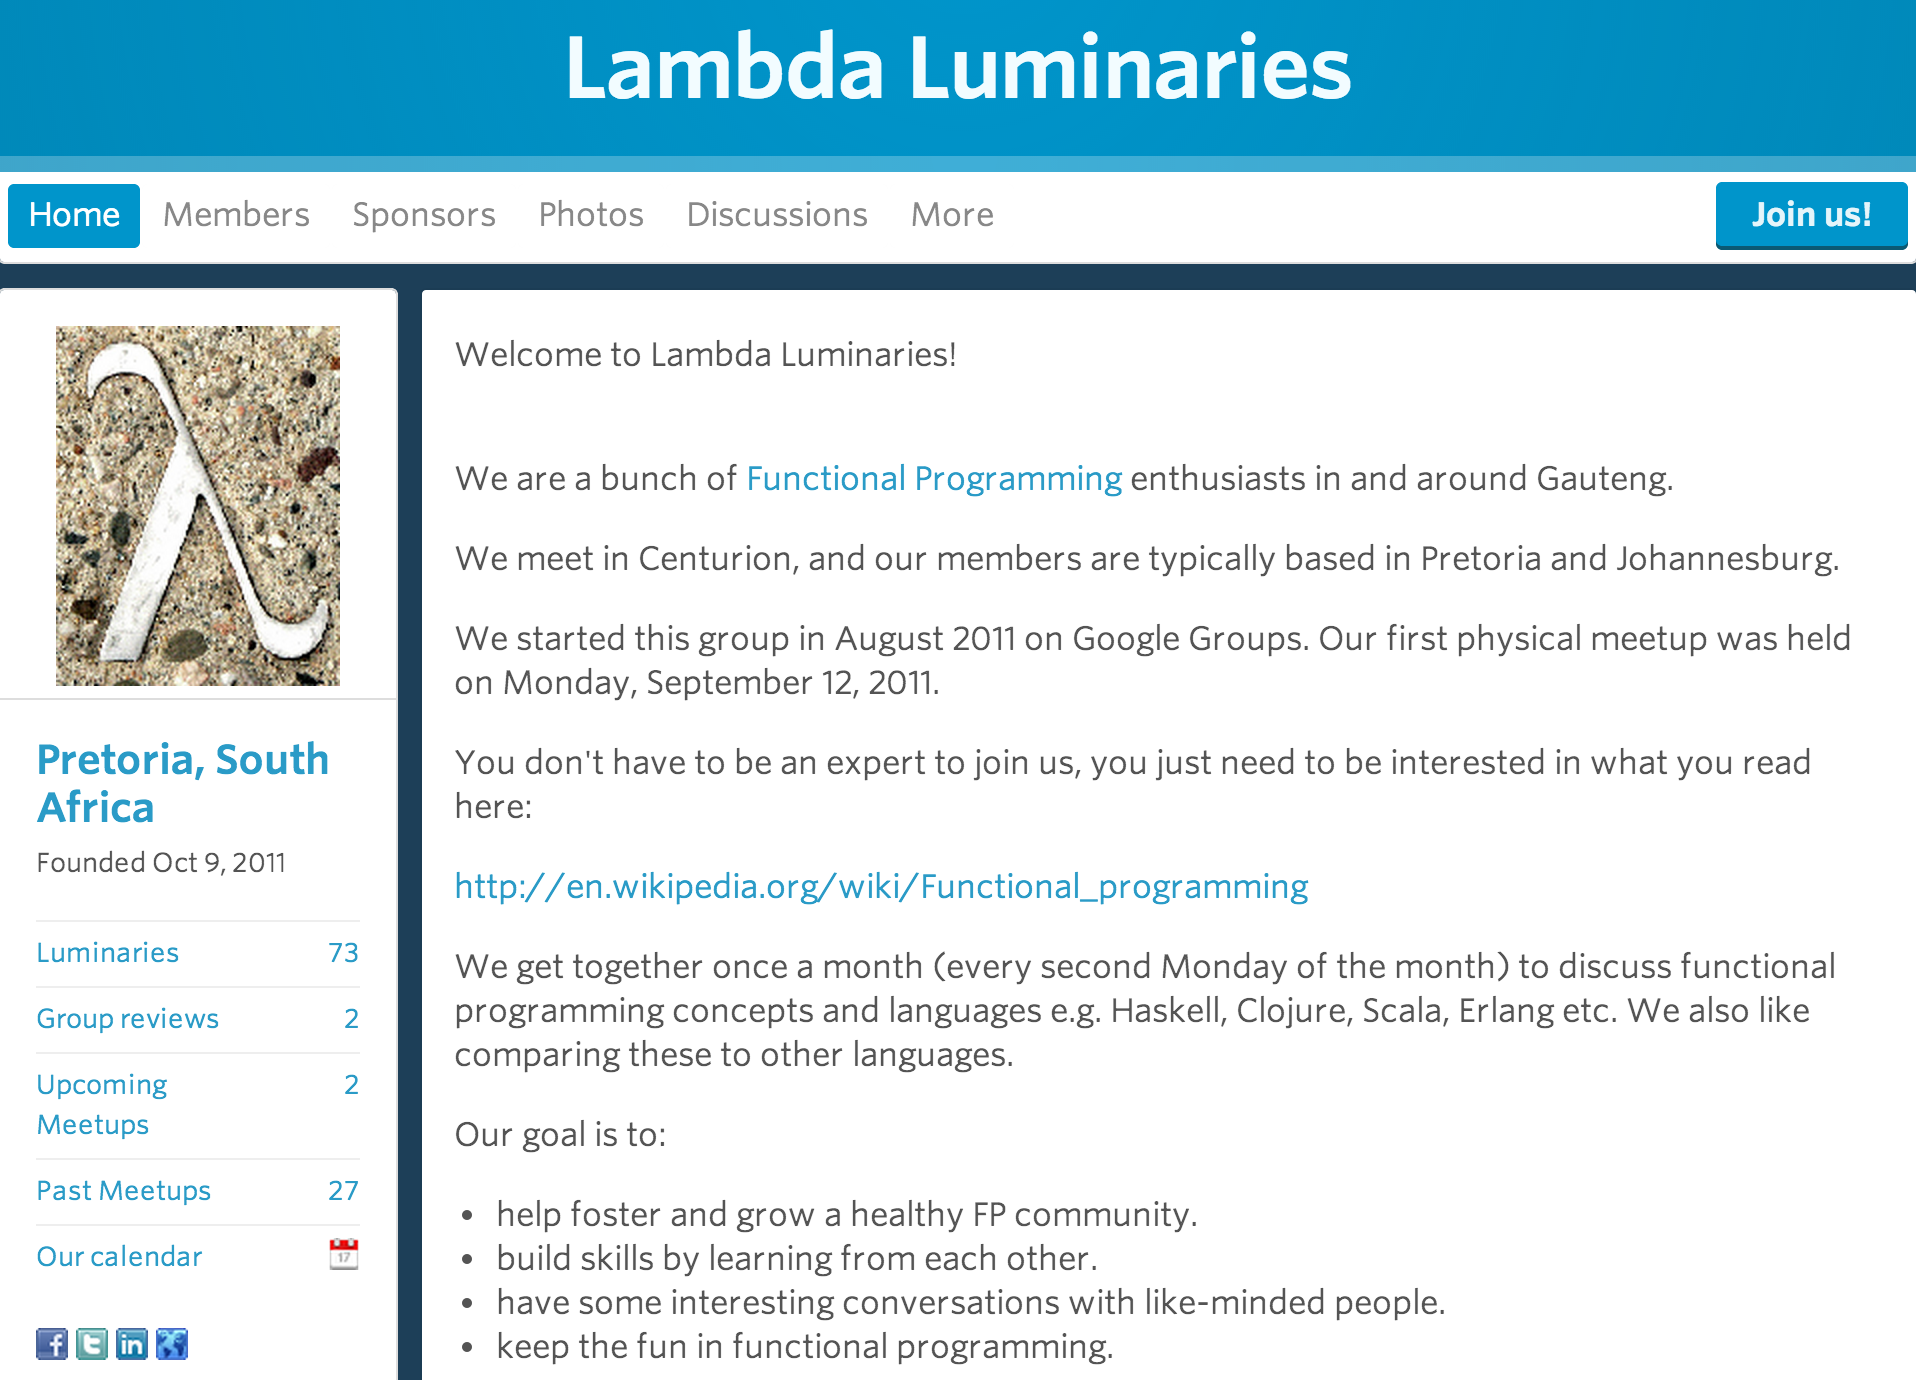
\includegraphics[scale=0.2]{img/ScreenShotLambdaLuminaries.png}
  \end{center}
  \url{http://www.meetup.com/lambda-luminaries/}
\end{frame}

\begin{frame}{Jemstep}
  \begin{center}
    
\includegraphics[scale=2]{img/Jemstep_HD_RGB.eps}
  \end{center}

  Retirement portfolio analysis in Scala.

  \vskip5mm

  \url{http://www.jemstep.com/}
\end{frame}

\section{Introduction}
\subsection{Introduction}

\begin{frame}
  \begin{center}
    
\includegraphics[scale=0.3]{img/cufp.png}
  \end{center}
\end{frame}

\begin{frame}
  \begin{center}
    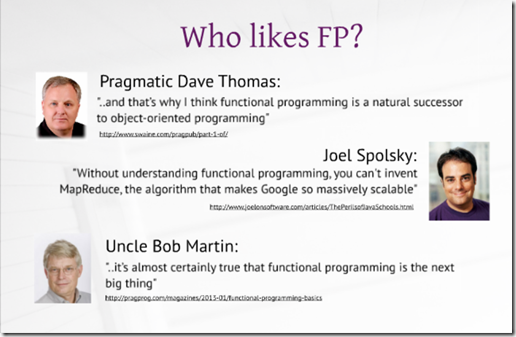
\includegraphics[scale=0.8]{img/WhoLikesFP.png}
  \end{center}
\end{frame}

\begin{frame}
  \begin{exampleblock}{}
    {\Large ``
      No matter what language you work in, programming
      in a functional style provides benefits.
      You should do it whenever it is convenient, and you
      should think hard about the decision when it isn’t convenient.
      ''}
    \vskip5mm
    \hspace*\fill{\small--- John Carmack, ID Software \cite{carmack}}
  \end{exampleblock}
\end{frame}

\begin{frame}{Quake}
  \begin{center}
    
\includegraphics[scale=0.3]{img/quake.png}
  \end{center}
\end{frame}

\begin{frame}

  \begin{center}
  {\Huge But what exactly is ``Functional Programming''?}
  \end{center}

\end{frame}

\section{Definition}
\subsection{Definition}

\begin{frame}{Functional Programming, noun:}

  \begin{exampleblock}{}
    {\Huge
      Functional Programming is a list of things you CAN’T do.
      }
    \vskip5mm
    \hspace*\fill{\small \cite{pauleyfp}}
  \end{exampleblock}
\end{frame}


\begin{frame}[fragile]{You can't vary your variables}
  \begin{minted}[fontsize=\Huge]{erl}
1> X = 42.
42
2> X = X + 1.
** exception error:
   no match of right hand
   side value 43
  \end{minted}
\end{frame}

\begin{frame}[fragile]{No while/for loops. Sorry :-(}
  \begin{minted}[fontsize=\Huge]{java}
int i;
for (i=1; i<=3; i++) {
  System.out.println(i);
}
  \end{minted}
\end{frame}

\begin{frame}[fragile]{You can't mutate/change your data structures}
     \begin{columns}[t]
     \begin{column}[T]{5cm}
Python
\begin{minted}[fontsize=\large]{python}
>>> list1 = [1,2,3]
>>> list2 = list1
>>> print list1.reverse()
None
>>> list1
[3, 2, 1]
>>> list2
[3, 2, 1]
\end{minted}
     \end{column}

     \begin{column}[T]{5cm}
Haskell
\begin{minted}[fontsize=\large]{haskell}
> let list1 = [1,2,3]
> let list2 = list1
> reverse(list1)
[3,2,1]
> list1
[1,2,3]
> list2
[1,2,3]
\end{minted}
     \end{column}
     \end{columns}
\end{frame}

\begin{frame}{You can't have any side effects}
  \begin{center}
    
\includegraphics[scale=0.4]{img/side-effects-cartoon.jpg}
  \end{center}
\end{frame}

\begin{frame}{Are you kidding me?}
  How can anyone program like this???
  \begin{center}
    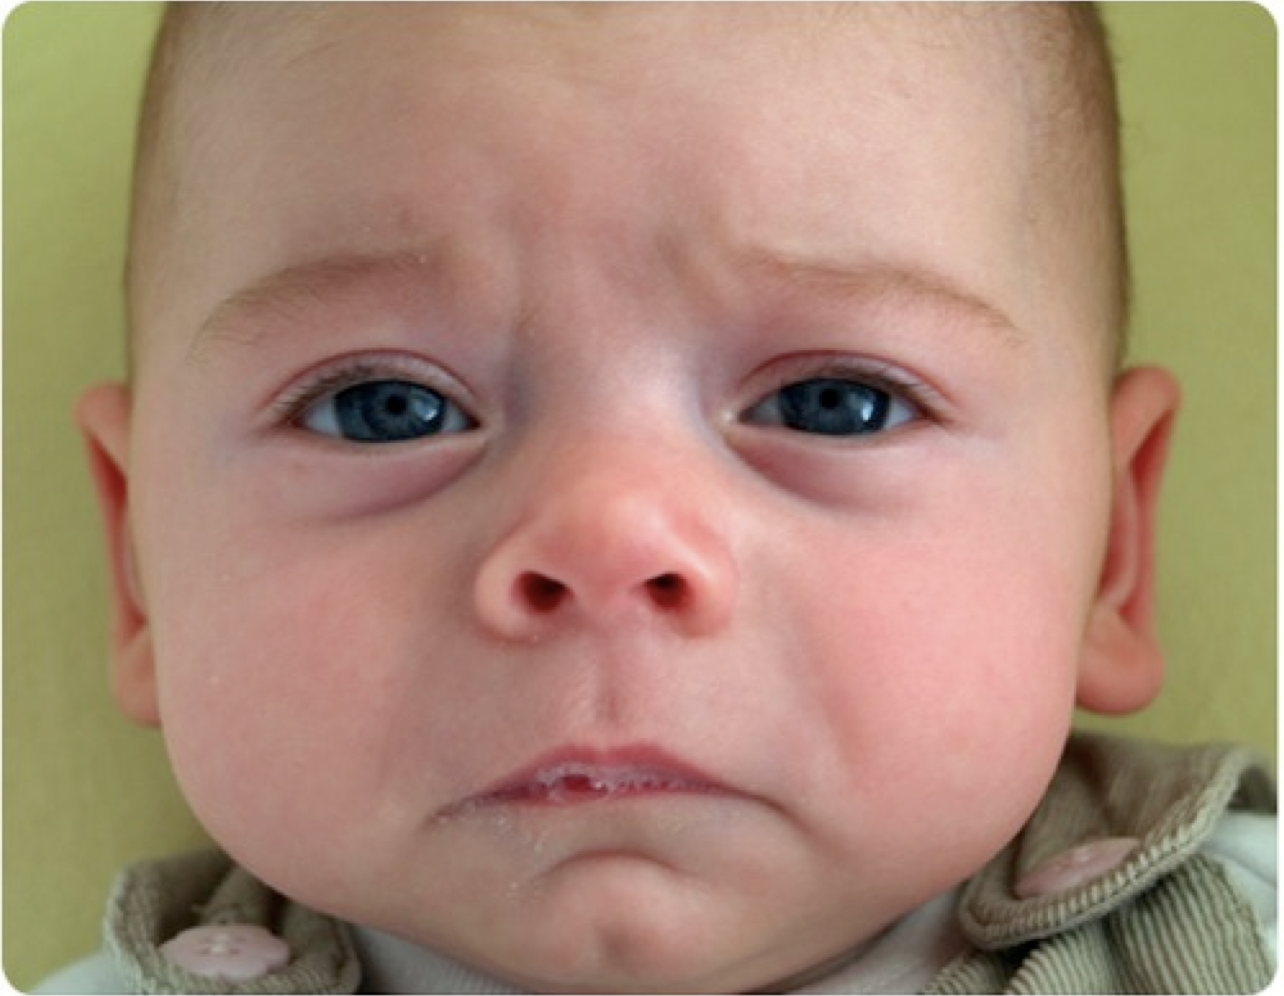
\includegraphics[scale=0.3]{img/sadbaby.png}
  \end{center}
\end{frame}

\begin{frame}{GOTO 10}
    This sounds like
  \begin{exampleblock}{}
    {\Large ``You can't have GOTO statements''}
  \end{exampleblock}
  \vskip5mm
  \hspace*\fill{\small See Hughes and Dijkstra \cite{whyfp, dijkstra}}
\end{frame}

\begin{frame}{}

  \begin{center}
    {\Huge It's not about what we cannot do.}
  \end{center}

\end{frame}

\begin{frame}{}

  \begin{center}
    {\Huge We need a better definition of Functional Programming.}
  \end{center}

\end{frame}

\begin{frame}{Programming Paradigms}
  \framesubtitle{(Very Simplified)}
  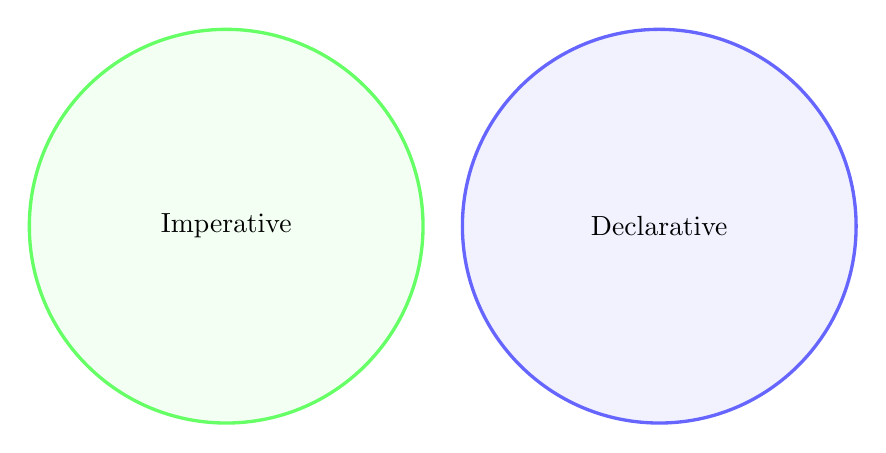
\begin{tikzpicture}[
      bluecircle/.style={circle,  draw=blue!60, fill=blue!5, very thick, minimum size=5cm},
      greencircle/.style={circle, draw=green!60, fill=green!5, very thick, minimum size=5cm}]

    \node[greencircle] (imperative)  at (0,3) {};
    \node[bluecircle]  (declarative) at (5.5,3) {};

    \node (i) at (0,3) {Imperative};
    \node (d) at (5.5,3) {\alert{Declarative}};
  \end{tikzpicture}
\end{frame}

\begin{frame}{Functional Programming, noun:}

\begin{exampleblock}{}
  {\Large ``
  Functional programming is so called because a program consists entirely of \alert{functions}.
  ''}
  \vskip5mm
  \hspace*\fill{\small--- John Hughes, Why Functional Programming
    Matters \cite[p.~1]{whyfp}}
\end{exampleblock}
\end{frame}

\begin{frame}{}

  {\Large OK... so what exactly is a \alert{function}?}

\end{frame}

\section{Function Recap}
\subsection{Function Recap}

\begin{frame}{An example function}

  {\Huge $f(x) = 2x^2 - 2x + 3$}

  \begin{tikzpicture}
    \begin{axis}[mypgfstyle]
      \addplot[domain=-1:3, color=blue] {2*(x^2) - (2*x) + 3};
    \end{axis}
  \end{tikzpicture}

\end{frame}

\begin{frame}{Variables in functions}

  {\Huge $f(x) = 2x^2 - 2x + 3$}

  \vskip5mm

When we evaluate the function:\\
$f(2) = 8 - 4 + 3 = 7$

  \begin{itemize}[<+->]
    \item The value of $x$ will not change inside the function body.
    \item Same input, same output. Every time. (Referential Transparency)
    \item We can call $f$ multiple times without any side effects (Idempotence).
    \item We don't have to recalculate $f(2)$, we can replace any
      occurrence of $f(2)$ with $7$ (Memoization).
  \end{itemize}
\end{frame}

\begin{frame}{Varying variables does not make sense}

  {\Huge
    \begin{align*}
           x     & = x + 1\\
           x - x & = 1\\
           0     & = 1\\
\therefore x     & \neq x + 1
    \end{align*}
  }

\end{frame}

\begin{frame}{Functions can call other functions}

  {\Huge $g(x) = f(x) + 1$}

\end{frame}

\begin{frame}[fragile]{Values are functions}

  {\large Constant values are just functions with no input parameters}

  \vskip5mm
  {\Huge $x = 42$}
  \vskip10mm

  \begin{columns}[t]
    \begin{column}[T]{5cm}
      Python function definition:
      \begin{minted}[fontsize=\Large]{python}
def x():
    return 42
      \end{minted}
    \end{column}

    \begin{column}[T]{5cm}
       Haskell function definition:
       \begin{minted}[fontsize=\Large]{haskell}
x = 42
       \end{minted}
    \end{column}
  \end{columns}
\end{frame}

\begin{frame}{Functions can be composed}

  {\Huge $h(x) = (f \circ g)(x) = f(g(x))$\\
  \vskip5mm
  or\\
  \vskip5mm
  $h = f \circ g$}

\end{frame}

\begin{frame}{Higher-order Functions}

  {\Large Functions can take functions as input.}\\
  {\Large Functions can return functions as the result.}

  \vskip5mm

  {\Huge $h(f, g, x) = f(x) + g(2)$}

\end{frame}

\begin{frame}{Higher-order Functions}

  {\Large The derivative of $f(x)$ returns another function.}

  \vskip5mm

  {\Large $f(x) = 2x^2 - 2x + 3$}\\
  {\Large $\frac{d}{dx} f(x) = 4x - 2$}

  \begin{tikzpicture}
    \begin{axis}[mypgfstyle]
      \addplot[domain=-1:3, color=blue] {2*(x^2) - (2*x) + 3};
      \addplot[domain=-1:3, color=magenta] {4*x - 2};
    \end{axis}
  \end{tikzpicture}

\end{frame}

\begin{frame}[fragile]{A functional program consists entirely of functions}

  \inputminted[firstline=6,lastline=15]{python}{code/python/justfunctions.py}

  \begin{verbatim}
$ ./justfunctions.py Hello from Python
2014-02-15 10:36:42.062697 Hello-from-Python
  \end{verbatim}

\end{frame}

\begin{frame}[fragile]{A functional program consists entirely of functions}

  \inputminted[firstline=5]{haskell}{code/haskell/justfunctions.hs}

  \begin{verbatim}
$ ./justfunctions Hello from Haskell
2014-02-15 08:36:50.822728 UTC Hello-from-Haskell
  \end{verbatim}

\end{frame}

\begin{frame}{Some Haskell Syntax}

  Python:
  \inputminted[fontsize=\large,firstline=11,lastline=12]{python}{code/python/justfunctions.py}
  \vskip5mm
  Haskell:
  \inputminted[fontsize=\large,firstline=11,lastline=13]{haskell}{code/haskell/justfunctions.hs}

\end{frame}

\section{Common Idioms}
\subsection{Recursion}

\begin{frame}[fragile]{Recursive function: Haskell}

  \inputminted[fontsize=\Large,lastline=3]{haskell}{code/haskell/doubleall_recursion.hs}

  \vskip5mm

Example use in the interactive interpreter:
  \begin{minted}[fontsize=\Large]{haskell}
Prelude Main> doubleAll [8,2,3]
[16,4,6]
  \end{minted}

\end{frame}

\begin{frame}[fragile]{Recursive function expanded}

  \inputminted[fontsize=\Large,firstline=2,lastline=3]{haskell}{code/haskell/doubleall_recursion.hs}

  \vskip5mm

  \begin{minted}[fontsize=\Large]{haskell}
doubleAll [8,2,3]
16 : (doubleAll [2,3])
16 : 4 : (doubleAll [3])
16 : 4 : 6 : (doubleAll [])
16 : 4 : 6 : []
16 : 4 : [6]
16 : [4,6]
[16,4,6]
  \end{minted}

\end{frame}

\begin{frame}[fragile]{Recursive function: Python}

  \inputminted[fontsize=\large,firstline=3,lastline=9]{python}{code/python/doubleall_recursion.py}

  \vskip5mm

Example use in the interactive interpreter:

  \begin{minted}[fontsize=\large]{python}
>>> doubleAll([8,2,3])
[16, 4, 6]
  \end{minted}

\end{frame}

\subsection{Pattern Matching}

\begin{frame}{Pattern Matching: Haskell}

  \inputminted[fontsize=\Large,lastline=3]{haskell}{code/haskell/doubleall_recursion.hs}

\end{frame}

\subsection{Higher-order Functions}

\begin{frame}{Higher-order Functions}
  \framesubtitle{3 Basic List Operations}

  \begin{description}[<+->]
  \item[Map] Convert each element of a list into some other value.
  \item[Filter] Get a subset of a list based on some condition.
  \item[Fold] Reduce a list of items to a single value.
  \end{description}

\end{frame}

\begin{frame}[fragile]{Map}

  Apply a function to each element of a list, and you get a new list.
  \vskip5mm
  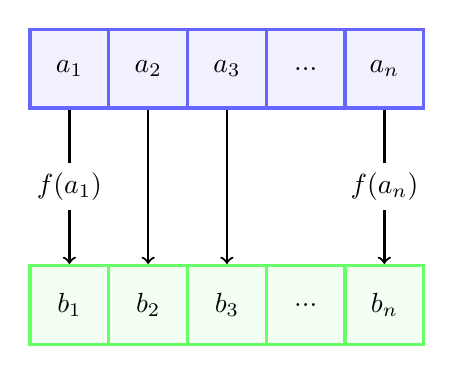
\begin{tikzpicture}[
      bluesquare/.style={rectangle,  draw=blue!60, fill=blue!5, very
        thick, minimum size=1cm},
      greensquare/.style={rectangle, draw=green!60, fill=green!5, very thick, minimum size=1cm}]

    \node[bluesquare] (a1) at (0,3) {$a_1$};
    \node[bluesquare] (a2) at (1,3) {$a_2$};
    \node[bluesquare] (a3) at (2,3) {$a_3$};
    \node[bluesquare] (ad) at (3,3) {$...$};
    \node[bluesquare] (an) at (4,3) {$a_n$};

    \node[greensquare] (b1) at (0,0) {$b_1$};
    \node[greensquare] (b2) at (1,0) {$b_2$};
    \node[greensquare] (b3) at (2,0) {$b_3$};
    \node[greensquare] (bd) at (3,0) {$...$};
    \node[greensquare] (bn) at (4,0) {$b_n$};

    \node (fa1) at (0,1.5) {$f(a_1)$};
    \node (fan) at (4,1.5) {$f(a_n)$};

    \draw[thick]    (a1)  -- (fa1);
    \draw[->,thick] (fa1) -- (b1);

    \draw[->,thick] (a2) -- (b2);
    \draw[->,thick] (a3) -- (b3);

    \draw[thick]    (an)  -- (fan);
    \draw[->,thick] (fan) -- (bn);

  \end{tikzpicture}

\end{frame}

\begin{frame}[fragile]{Map}

The built-in Haskell map function:

\begin{minted}[fontsize=\huge]{haskell}
map :: (a -> b) -> [a] -> [b]
map _ []     = []
map f (x:xs) = f x : map f xs
  \end{minted}

\end{frame}

\begin{frame}[fragile]{Map}

The builtin Haskell map function:
\begin{minted}[fontsize=\Large]{haskell}
map :: (a -> b) -> [a] -> [b]
map _ []     = []
map f (x:xs) = f x : map f xs
  \end{minted}

  \vskip5mm

Hmmm, looks very similar to our previous doubleAll function:

\inputminted[fontsize=\Large,lastline=3]{haskell}{code/haskell/doubleall_recursion.hs}
\end{frame}

\begin{frame}[fragile]{Map}

So our doubleAll can actually be simplified.

  \vskip5mm

In Haskell:
\begin{minted}[fontsize=\Large]{haskell}
doubleAll = map (*2)
  \end{minted}

  \vskip5mm

In Python:
\inputminted[fontsize=\Large,firstline=3,lastline=4]{python}{code/python/doubleall_map.py}
\end{frame}

\begin{frame}[fragile]{Map}

  \begin{minted}[fontsize=\Large]{haskell}
doubleAll :: Num a => [a] -> [a]
doubleAll = map (*2)
  \end{minted}

  \vskip5mm

  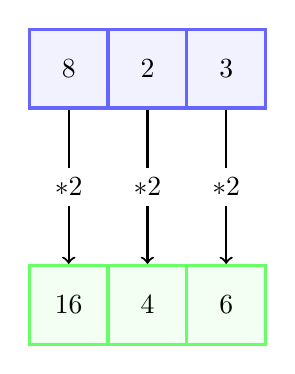
\begin{tikzpicture}[
      bluesquare/.style={rectangle,  draw=blue!60, fill=blue!5, very
        thick, minimum size=1cm},
      greensquare/.style={rectangle, draw=green!60, fill=green!5, very thick, minimum size=1cm}]

    \node[bluesquare] (a1) at (0,3) {$8$};
    \node[bluesquare] (a2) at (1,3) {$2$};
    \node[bluesquare] (a3) at (2,3) {$3$};

    \node[greensquare] (b1) at (0,0) {$16$};
    \node[greensquare] (b2) at (1,0) {$4$};
    \node[greensquare] (b3) at (2,0) {$6$};

    \node (fa1) at (0,1.5) {$*2$};
    \node (fa2) at (1,1.5) {$*2$};
    \node (fa3) at (2,1.5) {$*2$};

    \draw[thick]    (a1)  -- (fa1);
    \draw[->,thick] (fa1) -- (b1);

    \draw[thick]    (a2)  -- (fa2);
    \draw[->,thick] (fa2) -- (b2);

    \draw[thick]    (a3)  -- (fa3);
    \draw[->,thick] (fa3) -- (b3);

  \end{tikzpicture}

\end{frame}

\begin{frame}{Account Data}

  \inputminted[fontsize=\large,firstline=3,lastline=3]{haskell}{code/haskell/accounts.hs}
  \inputminted[fontsize=\large,firstline=19,lastline=22]{haskell}{code/haskell/accounts.hs}

\end{frame}

\begin{frame}{Account Data}

  \inputminted[fontsize=\small,firstline=28,lastline=43,gobble=11]{haskell}{code/haskell/accounts.hs}

\end{frame}

\begin{frame}{Map}

  Map on account data:
  \inputminted[fontsize=\Large,firstline=45,lastline=46]{haskell}{code/haskell/accounts.hs}

  \vskip5mm

  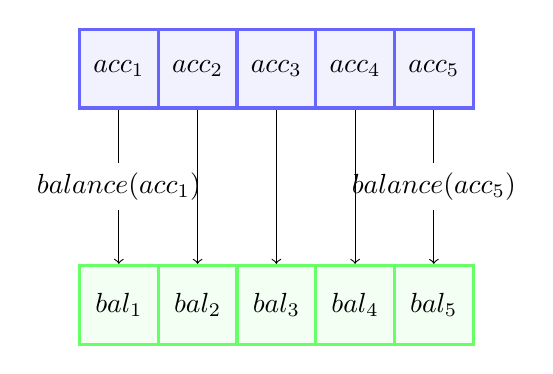
\begin{tikzpicture}[
      bluesquare/.style={rectangle,  draw=blue!60, fill=blue!5, very
        thick, minimum size=1cm},
      greensquare/.style={rectangle, draw=green!60, fill=green!5, very thick, minimum size=1cm}]

    \node[bluesquare] (a1) at (0,3) {$acc_1$};
    \node[bluesquare] (a2) at (1,3) {$acc_2$};
    \node[bluesquare] (a3) at (2,3) {$acc_3$};
    \node[bluesquare] (a4) at (3,3) {$acc_4$};
    \node[bluesquare] (a5) at (4,3) {$acc_5$};

    \node[greensquare] (b1) at (0,0) {$bal_1$};
    \node[greensquare] (b2) at (1,0) {$bal_2$};
    \node[greensquare] (b3) at (2,0) {$bal_3$};
    \node[greensquare] (b4) at (3,0) {$bal_4$};
    \node[greensquare] (b5) at (4,0) {$bal_5$};

    \node (fa1) at (0,1.5) {$balance(acc_1)$};
    \node (fa5) at (4,1.5) {$balance(acc_5)$};

    \draw     (a1)  -- (fa1);
    \draw[->] (fa1) -- (b1);

    \draw[->] (a2) -- (b2);
    \draw[->] (a3) -- (b3);
    \draw[->] (a4) -- (b4);

    \draw     (a5)  -- (fa5);
    \draw[->] (fa5) -- (b5);

  \end{tikzpicture}

\end{frame}

\begin{frame}{Filter}

\begin{center}
  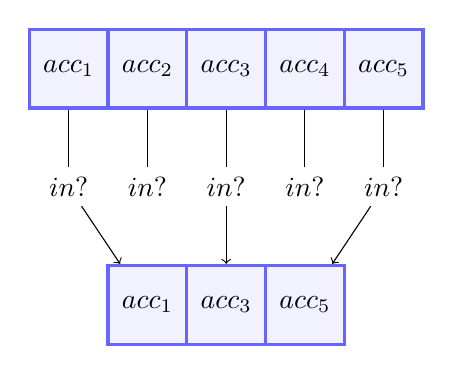
\begin{tikzpicture}[
      bluesquare/.style={rectangle,  draw=blue!60, fill=blue!5, very
        thick, minimum size=1cm}]

    \node[bluesquare] (a1) at (0,3) {$acc_1$};
    \node[bluesquare] (a2) at (1,3) {$acc_2$};
    \node[bluesquare] (a3) at (2,3) {$acc_3$};
    \node[bluesquare] (a4) at (3,3) {$acc_4$};
    \node[bluesquare] (a5) at (4,3) {$acc_5$};

    \node[bluesquare] (b1) at (1,0) {$acc_1$};
    \node[bluesquare] (b2) at (2,0) {$acc_3$};
    \node[bluesquare] (b3) at (3,0) {$acc_5$};

    \node (fa1) at (0,1.5) {$in?$};
    \node (fa2) at (1,1.5) {$in?$};
    \node (fa3) at (2,1.5) {$in?$};
    \node (fa4) at (3,1.5) {$in?$};
    \node (fa5) at (4,1.5) {$in?$};

    \draw (a1) -- (fa1);
    \draw (a2) -- (fa2);
    \draw (a3) -- (fa3);
    \draw (a4) -- (fa4);
    \draw (a5) -- (fa5);

    \draw[->] (fa1) -- (b1);
    \draw[->] (fa3) -- (b2);
    \draw[->] (fa5) -- (b3);

  \end{tikzpicture}
\end{center}
\end{frame}

\begin{frame}[fragile]{Filter}

Filter on account data:
\inputminted[fontsize=\large,firstline=48,lastline=52]{haskell}{code/haskell/accounts.hs}

  \vskip5mm

Output:
  \begin{verbatim}
*Main> topAccounts accounts
[FNB 6868773585 (J. Black) R5782347.99,
 FNB 6584539813 (S. Jones) R2937361.45]
  \end{verbatim}

\end{frame}

\begin{frame}[fragile]{Fold/Reduce/Inject}
  \begin{columns}[t]

    \begin{column}[T]{5cm}

      \begin{minted}[fontsize=\Large]{haskell}
foldl (+) 0 [8,2,3]
13
      \end{minted}
    \end{column}

    \begin{column}[T]{5cm}

      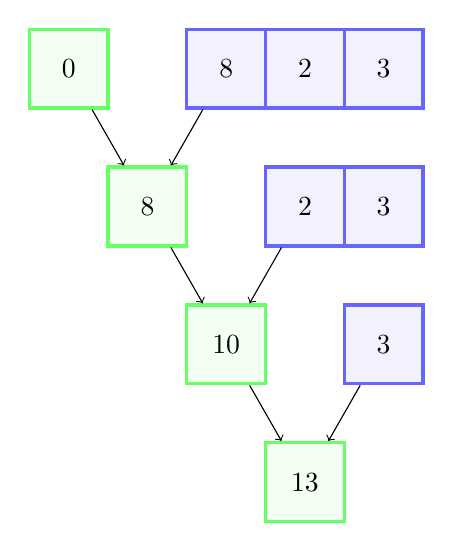
\begin{tikzpicture}[
          bluesquare/.style={rectangle,  draw=blue!60, fill=blue!5, very
            thick, minimum size=1cm},
          greensquare/.style={rectangle, draw=green!60, fill=green!5, very thick, minimum size=1cm}]

        \node[greensquare] (acc0) at (0,8) {0};
        \node[bluesquare]  (a1)   at (2,8) {8};
        \node[bluesquare]         at (3,8) {2};
        \node[bluesquare]         at (4,8) {3};

        \node[greensquare] (acc1) at (1,6.25) {8};
        \node[bluesquare]  (a2)   at (3,6.25) {2};
        \node[bluesquare]         at (4,6.25) {3};

        \draw[->] (acc0) -- (acc1);
        \draw[->] (a1)   -- (acc1);

        \node[greensquare] (acc2) at (2,4.5) {10};
        \node[bluesquare]  (a3)   at (4,4.5) {3};

        \draw[->] (acc1) -- (acc2);
        \draw[->] (a2)   -- (acc2);

        \node[greensquare] (acc3) at (3,2.75) {13};

        \draw[->] (acc2) -- (acc3);
        \draw[->] (a3)   -- (acc3);

      \end{tikzpicture}
    \end{column}
  \end{columns}

\end{frame}

\begin{frame}[fragile]{Fold/Reduce/Inject}
      \begin{minted}[fontsize=\Large]{haskell}
foldl (+) 0 (balances accounts)
      \end{minted}

      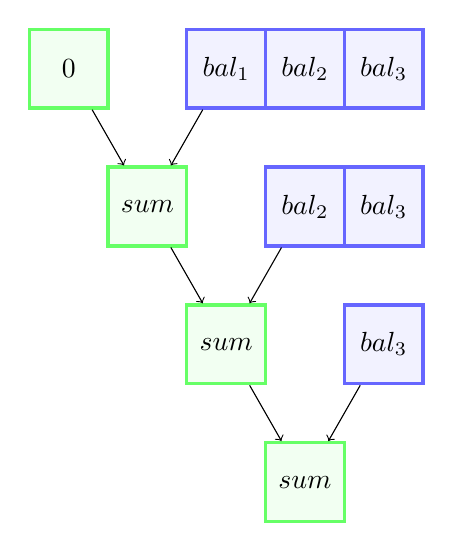
\begin{tikzpicture}[
          bluesquare/.style={rectangle,  draw=blue!60, fill=blue!5, very
            thick, minimum size=1cm},
          greensquare/.style={rectangle, draw=green!60, fill=green!5, very thick, minimum size=1cm}]

        \node[greensquare] (acc0) at (0,8) {0};
        \node[bluesquare]  (a1)   at (2,8) {$bal_1$};
        \node[bluesquare]         at (3,8) {$bal_2$};
        \node[bluesquare]         at (4,8) {$bal_3$};

        \node[greensquare] (acc1) at (1,6.25) {$sum$};
        \node[bluesquare]  (a2)   at (3,6.25) {$bal_2$};
        \node[bluesquare]         at (4,6.25) {$bal_3$};

        \draw[->] (acc0) -- (acc1);
        \draw[->] (a1)   -- (acc1);

        \node[greensquare] (acc2) at (2,4.5) {$sum$};
        \node[bluesquare]  (a3)   at (4,4.5) {$bal_3$};

        \draw[->] (acc1) -- (acc2);
        \draw[->] (a2)   -- (acc2);

        \node[greensquare] (acc3) at (3,2.75) {$sum$};

        \draw[->] (acc2) -- (acc3);
        \draw[->] (a3)   -- (acc3);

      \end{tikzpicture}
\end{frame}

\begin{frame}[fragile]{balancesPerBank}
      \begin{minted}[fontsize=\Large]{haskell}
foldl insertBalance Map.empty accounts
      \end{minted}

      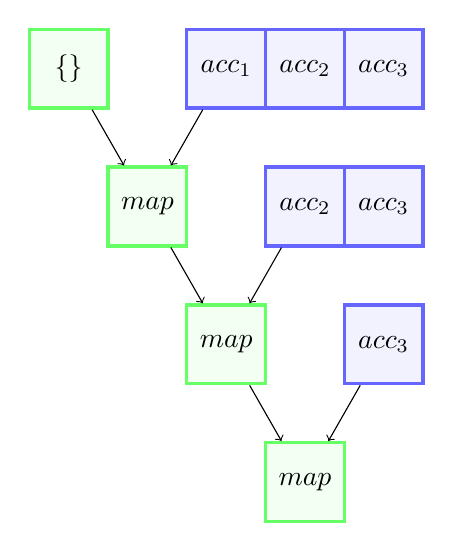
\begin{tikzpicture}[
          bluesquare/.style={rectangle,  draw=blue!60, fill=blue!5, very
            thick, minimum size=1cm},
          greensquare/.style={rectangle, draw=green!60, fill=green!5, very thick, minimum size=1cm}]

        \node[greensquare] (acc0) at (0,8) {\{\}};
        \node[bluesquare]  (a1)   at (2,8) {$acc_1$};
        \node[bluesquare]         at (3,8) {$acc_2$};
        \node[bluesquare]         at (4,8) {$acc_3$};

        \node[greensquare] (acc1) at (1,6.25) {$map$};
        \node[bluesquare]  (a2)   at (3,6.25) {$acc_2$};
        \node[bluesquare]         at (4,6.25) {$acc_3$};

        \draw[->] (acc0) -- (acc1);
        \draw[->] (a1)   -- (acc1);

        \node[greensquare] (acc2) at (2,4.5) {$map$};
        \node[bluesquare]  (a3)   at (4,4.5) {$acc_3$};

        \draw[->] (acc1) -- (acc2);
        \draw[->] (a2)   -- (acc2);

        \node[greensquare] (acc3) at (3,2.75) {$map$};

        \draw[->] (acc2) -- (acc3);
        \draw[->] (a3)   -- (acc3);

      \end{tikzpicture}
\end{frame}

\begin{frame}[fragile]{Fold}

  \inputminted[fontsize=\large,firstline=57,lastline=59]{haskell}{code/haskell/accounts.hs}

Output:
  \begin{verbatim}
*Main> balancesPerBank accounts
fromList [(ABSA,R123100.23),(FNB,R8719709.44)]
  \end{verbatim}

\end{frame}

\begin{frame}{Fold}

  \inputminted[fontsize=\small,firstline=57,lastline=71]{haskell}{code/haskell/accounts.hs}

\end{frame}

\section{Imperative Comparison}
\subsection{Imperative Comparison}

\begin{frame}{Programming Paradigms}
  \framesubtitle{(Very Simplified)}
  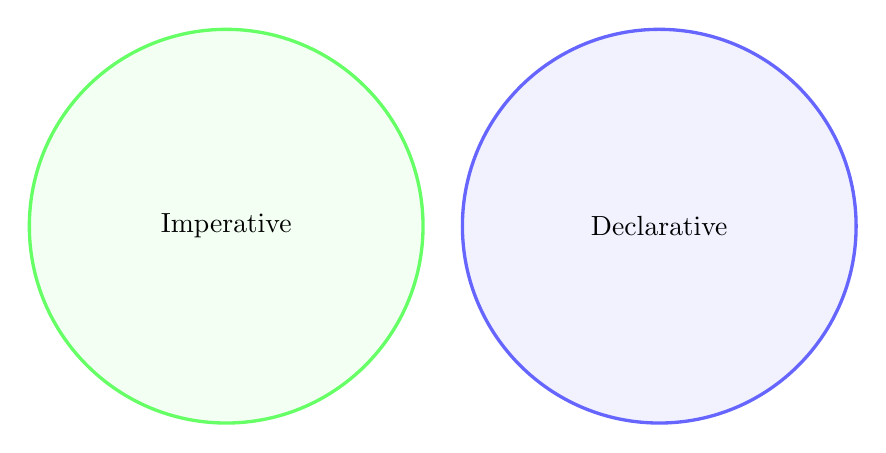
\begin{tikzpicture}[
      bluecircle/.style={circle,  draw=blue!60, fill=blue!5, very thick, minimum size=5cm},
      greencircle/.style={circle, draw=green!60, fill=green!5, very thick, minimum size=5cm}]

    \node[greencircle] (imperative)  at (0,3) {};
    \node[bluecircle]  (declarative) at (5.5,3) {};

    \node (i) at (0,3) {\alert{Imperative}};
    \node (d) at (5.5,3) {Declarative};
  \end{tikzpicture}
\end{frame}

\begin{frame}

  In imperative programming:

  \begin{itemize}[<+->]
  \item Your variables can vary any time!
  \item You have to use locks to be thread-safe!
  \item You have to write your own loops for the most basic list operations!
  \item Your data structures are mutable!
  \item You have to defensively make copies of data to prevent bugs!
  \item You have to defensively check for null values!
  \item You have to think about implicit state! (this, self)
  \item Code is generally riddled with side effects!
  \end{itemize}
\end{frame}

\begin{frame}{Are you kidding me?}
  How can anyone program like this???
  \begin{center}
    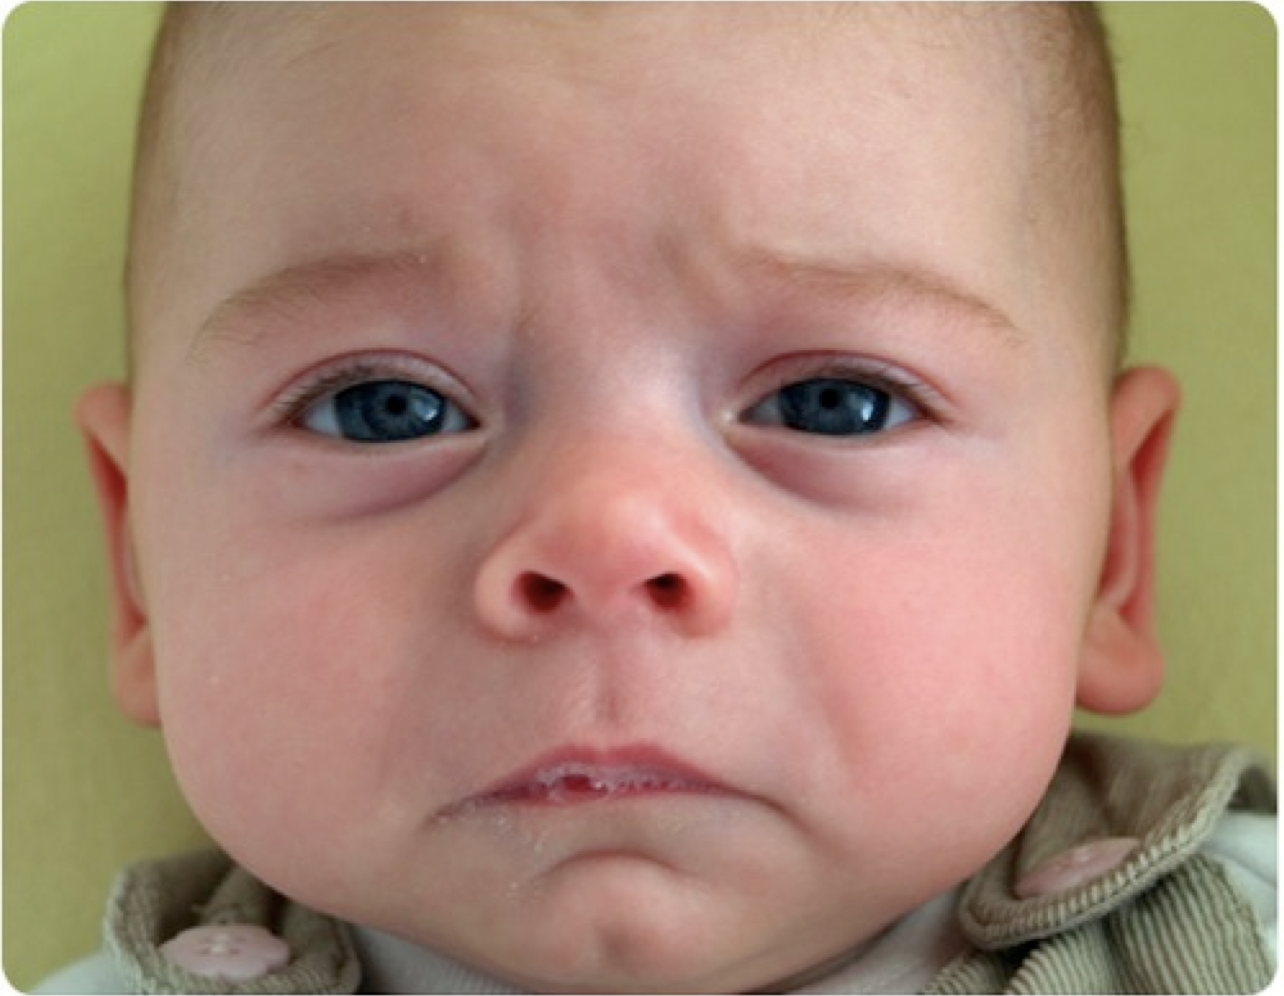
\includegraphics[scale=0.3]{img/sadbaby.png}
  \end{center}
\end{frame}

\section{Challenges!}
\subsection{Challenges!}

\begin{frame}
  \begin{center}
    
\includegraphics[scale=0.2]{img/AreYouReadyfortheChallenge.jpg}
  \end{center}
\end{frame}

\begin{frame}{Join the anti-for campaign}

  \begin{center}
    {\Huge Less loops, more map/filter/fold}
  \end{center}
  \vskip5mm
  \url{http://weblogs.asp.net/podwysocki/archive/2009/06/26/the-anti-for-campaign.aspx}
  
\end{frame}

\begin{frame}{Treat side effects as a first-class concern}

  \begin{center}
    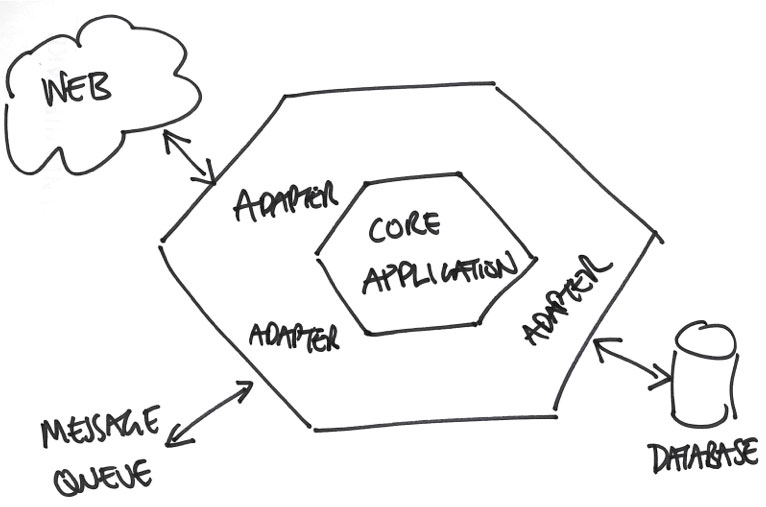
\includegraphics[scale=0.3]{img/hexagonal_architecture_sketch.jpg}
  \end{center}

\end{frame}

\begin{frame}{Learn a functional language}

\begin{exampleblock}{}
  {\Large ``
    A language that doesn't affect the way you think about programming, is not worth knowing.
  ''}
  \vskip5mm
  \hspace*\fill{\small--- Alan Perlis\cite{perlis19}}
\end{exampleblock}

\end{frame}

\begin{frame}{Disclaim your inheritance}

  {\Huge Write non-trivial code without using objects and inheritance.}
  \vskip5mm
  
  {\Large Get \alert{re-usability} with higher-order functions.}
  \vskip2mm
  {\Large Try to \alert{minimise moving parts} instead of encapsulating moving parts.}
  {\small\cite{mfeathers}}

\end{frame}

\begin{frame}{Join our group}
  \framesubtitle{@lambdaluminary}
  We meet once a month, on the second Monday of the month.

  \url{http://www.meetup.com/lambda-luminaries/}
  \begin{center}
    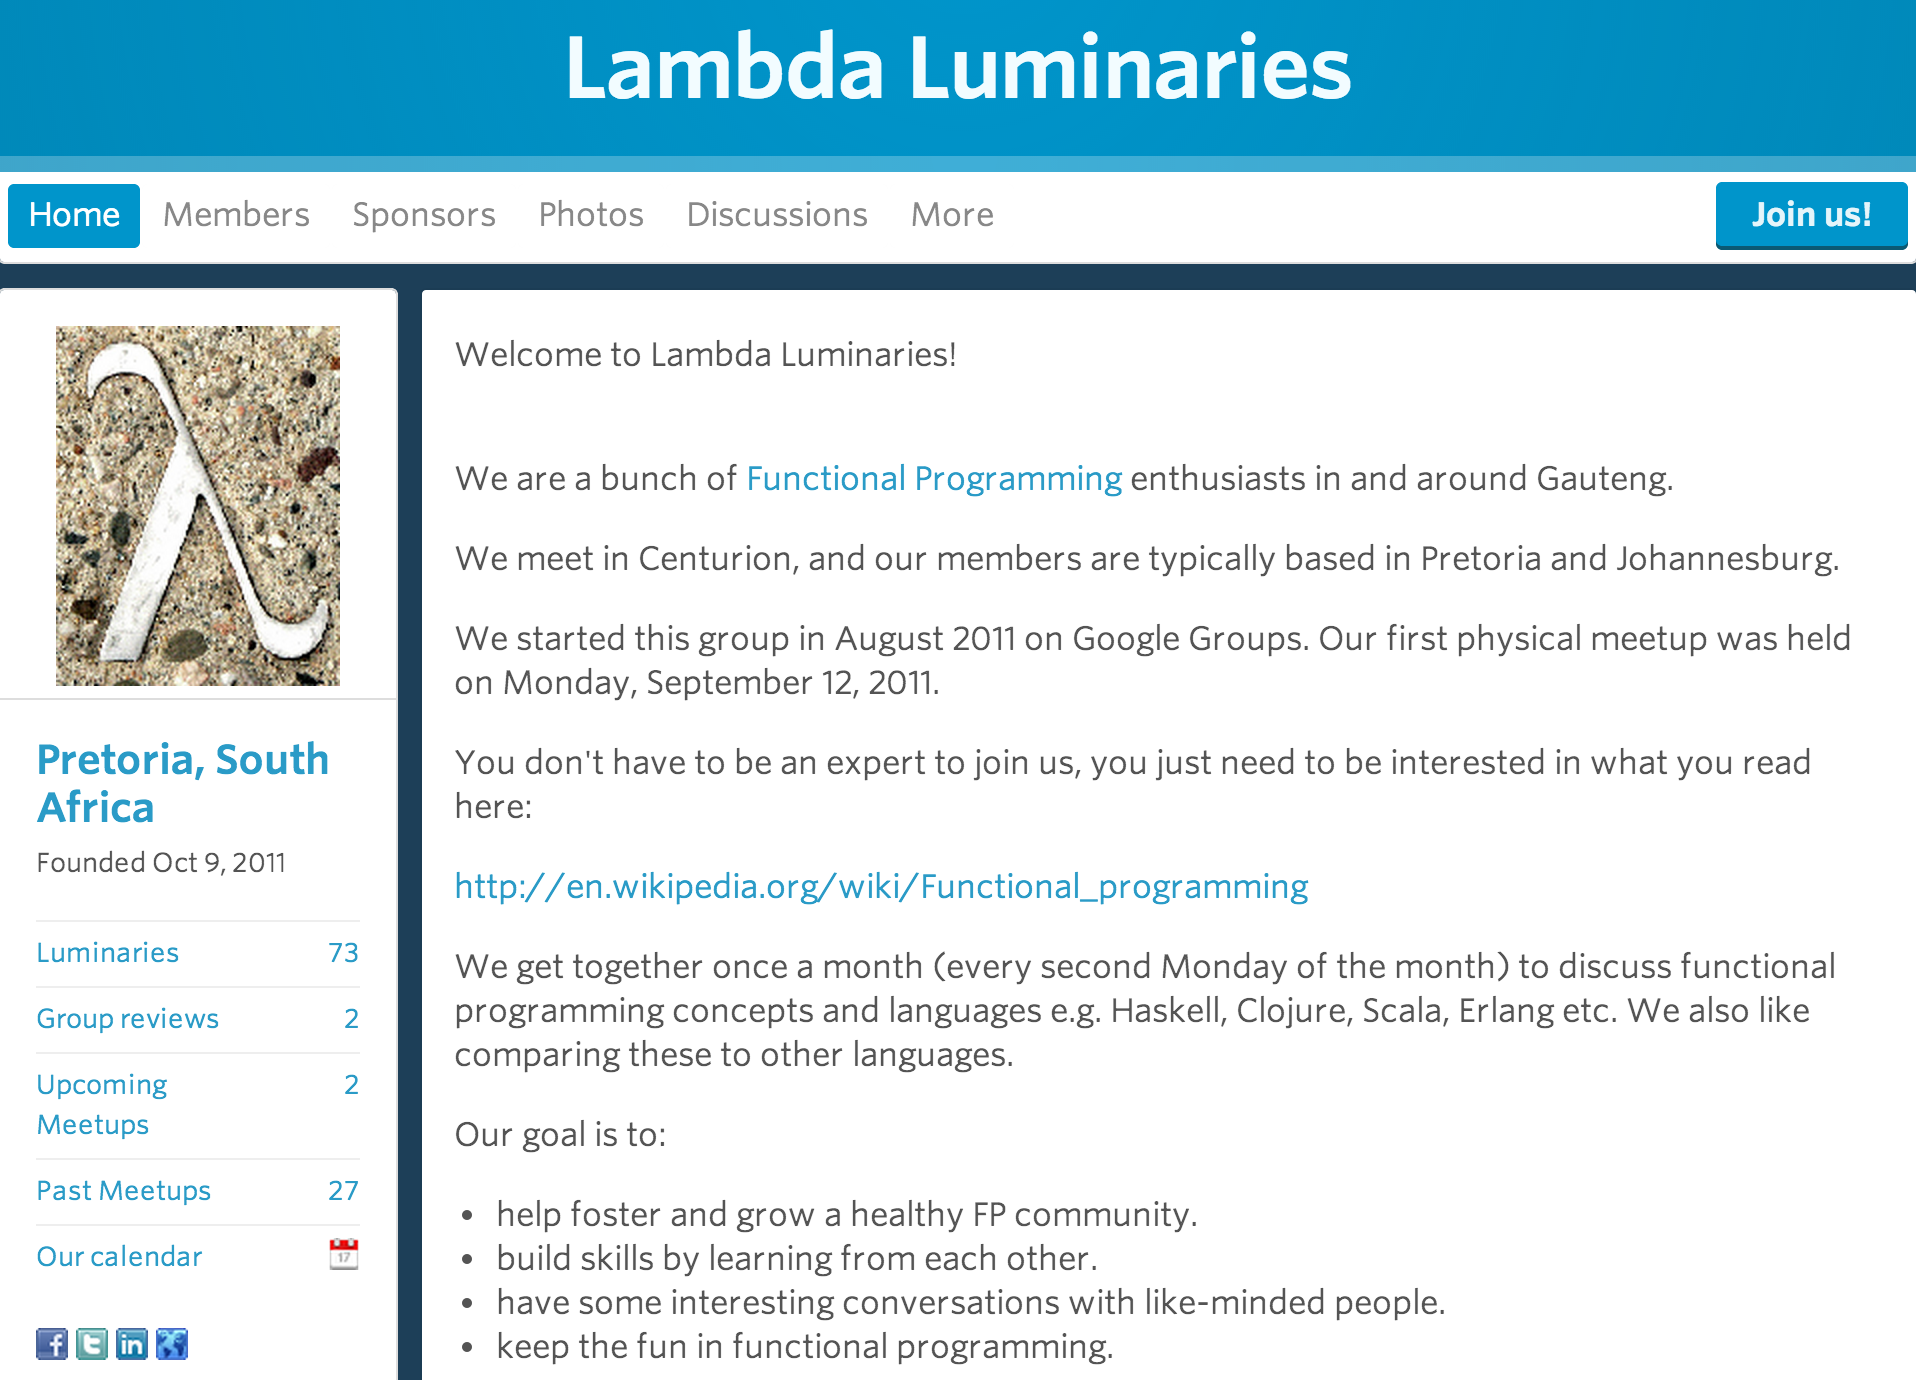
\includegraphics[scale=0.2]{img/ScreenShotLambdaLuminaries.png}
  \end{center}
\end{frame}

\begin{frame}{Get out of your comfort zone}

  {\Large Functional Programming is unfamiliar territory for most.}

\begin{exampleblock}{}
  {\Large ``
    If you want everything to be familiar you will never learn anything new.
  ''}
  \vskip5mm
  \hspace*\fill{\small--- Rich Hickey, author of Clojure\cite{hickey}}
\end{exampleblock}

\end{frame}

\section{Industry Use}
\subsection{Industry Use}

\begin{frame}{Companies In South Africa}

  \begin{description}
  \item[Jemstep, Sandton] Using Scala for Fund Analysis
  \item[Allan Gray, Cape Town] Using Scala for backend logic and system integration.
  \item[Yuppiechef, Cape Town] Using Clojure for their Warehouse
    Management System.
  \item[Cognician, Cape Town] Using Clojure to create coaching/learning modules.
  \item[Eldo Energy, Johannesburg] Using Clojure for automated meter
    reading and intelligent monitoring of consumer energy.
  \item[Rheo Systems, Pretoria] Using Clojure for supply chain integration.
  \end{description}

\end{frame}

\begin{frame}{Companies In South Africa}

  \begin{description}
  \item[Pattern Matched Technologies, Midrand] Using Erlang for all systems,
    eg. processing high volumes of financial transactions.
  \item[Effective Control Systems, Kyalami] Using Erlang for printer
    management.
  \item[Mira Networks, Somerset West] Using Erlang for billing
    administration and mobile development.
  \item[Kotive] Using Scala for designing workflow processes.
  \end{description}

\end{frame}

\section{Now what?}
\subsection{Now what?}

\begin{frame}{Online Courses}

  \begin{thebibliography}{10}
    \bibitem{fpthinkingnealford}
      Functional Thinking by Neal Ford
      \newblock O' Reilly
      \newblock \url{http://shop.oreilly.com/product/0636920030393.do}
    \bibitem{fpinscalacourse}
      Functional Programming Principles in Scala
      \newblock EPFL University
      \newblock \url{https://www.coursera.org/course/progfun}
    \bibitem{fpcomplete}
      School of Haskell
      \newblock FP Complete
      \newblock \url{https://www.fpcomplete.com/school}
    \bibitem{proglangcourse}
      Programming Languages
      \newblock University of Washington
      \newblock \url{https://www.coursera.org/course/proglang}
  \end{thebibliography}

\end{frame}

\begin{frame}{Books}

  \begin{thebibliography}{10}
    \bibitem{haskellforgreatgood}
      Miran Lipovača
      \newblock Learn You a Haskell for Great Good!
      \newblock \url{http://learnyouahaskell.com/}
    \bibitem{erlangforgreatgood}
      Fred Hébert
      \newblock Learn You Some Erlang for Great Good!
      \newblock \url{http://learnyousomeerlang.com/}
    \bibitem{rwocaml}
      Yaron Minski, Anil Madhavapeddy, Jason Hickey
      \newblock Real World OCaml
      \newblock \url{https://realworldocaml.org/}
    \bibitem{fpinscalabook}
      Paul Chiusano, Rúnar Bjarnason
      \newblock Functional Programming in Scala
      \newblock \url{http://www.manning.com/bjarnason/}
  \end{thebibliography}

\end{frame}

\begin{frame}[allowframebreaks]{References}
  \begin{thebibliography}{10}
    \bibitem{whyfp}
      John Hughes
      \newblock Why Functional Programming Matters
      \newblock \url{http://www.cs.kent.ac.uk/people/staff/dat/miranda/whyfp90.pdf}
    \bibitem{carmack}
      John Carmack
      \newblock Functional Programming in C++
      \newblock \url{http://www.altdevblogaday.com/2012/04/26/functional-programming-in-c/}
    \bibitem{dijkstra}
      Edsger W. Dijkstra
      \newblock Go To Statement Considered Harmful
      \newblock \url{http://www.u.arizona.edu/~rubinson/copyright_violations/Go_To_Considered_Harmful.html}
    \bibitem{mfeathers}
      Tweet by Michael Feathers
      \newblock \url{https://twitter.com/mfeathers/status/29581296216}
    \bibitem{perlis19}
      Alan Jay Perlis
      \newblock \url{http://www.cs.yale.edu/quotes.html}
    \bibitem{hickey}
      Rich Hickey
      \newblock \url{http://www.infoq.com/presentations/Simple-Made-Easy}
    \bibitem{pauleyfp}
      Andreas Pauley
      \newblock An Introduction to Functional Programming
      \newblock \url{https://github.com/apauley/fp_presentation}
  \end{thebibliography}
\end{frame}

\end{document}
